\documentclass[aspectratio=169,11pt]{beamer}

% ================================================================
% "TABIIY TILNI QAYTA ISHLASH" KURSI
% MA'RUZA 10 --- Nomlangan obyektlarni tanib olish (NER)
%              (d10_ner.tex)
% Arxetiplar: [A][B][C][D][E] + 4 tsikl [F][G][H][I][J][K][L] +
%             [M][N][O][P][Q][R] + ilova [S]
% Rendered slayd soni: ~45 (3-haftaning ikkinchi ma'ruzasi; L1-L9 chuqurligi)
% Qulflangan [I1]: IOB2 "Malika Toshkentda ishlaydi ." -> [B-PER, B-LOC, O, O]
%   --- P10 (Day 11) birinchi assert manbayi (course_map hand_example).
% ================================================================

% ================================================================
% RANGLAR  (asl fayldan o'zgarishsiz)
% ================================================================
\definecolor{cnublue}{rgb}{0.07,0.14,0.62}
\definecolor{cnubluelight}{rgb}{0.18,0.30,0.72}
\definecolor{cnubluebg}{rgb}{0.90,0.92,0.97}
\definecolor{deepblue}{rgb}{0.07,0.14,0.62}
\definecolor{deepred}{rgb}{0.60,0.00,0.00}
\definecolor{deepgreen}{rgb}{0.00,0.45,0.00}
\definecolor{halfgray}{gray}{0.55}

% ================================================================
% BEAMER MAVZU --- Boadilla + maxsus footer  (asl fayldan o'zgarishsiz)
% ================================================================
\usetheme{Boadilla}

\setbeamercolor{structure}{fg=cnublue}
\setbeamercolor{frametitle}{bg=cnublue,fg=white}
\setbeamercolor{title}{bg=cnublue,fg=white}
\setbeamercolor{block title}{bg=cnublue,fg=white}
\setbeamercolor{block body}{bg=cnubluebg,fg=black}
\setbeamercolor{alerted text}{fg=deepred}
\setbeamercolor{author in head/foot}{bg=cnubluelight,fg=white}
\setbeamercolor{section in head/foot}{bg=cnublue,fg=white}
\setbeamercolor{page number in head/foot}{bg=cnubluelight,fg=white}

\setbeamertemplate{mini frame}{}
\setbeamertemplate{mini frame in current section}{}
\setbeamertemplate{mini frame in current subsection}{}
\setbeamertemplate{headline}{}
\setbeamertemplate{navigation symbols}{}

\setbeamertemplate{footline}{%
  \leavevmode%
  \hbox{%
    \begin{beamercolorbox}[wd=0.17\paperwidth,ht=2.5ex,dp=1.25ex,leftskip=0.5em]{author in head/foot}%
      \usebeamerfont{author in head/foot}\scriptsize\insertshortauthor%
    \end{beamercolorbox}%
    \begin{beamercolorbox}[wd=0.69\paperwidth,ht=2.5ex,dp=1.25ex,center]{section in head/foot}%
      \usebeamerfont{section in head/foot}%
      \scriptsize\insertsectionnavigationhorizontal{0.69\paperwidth}{}{}%
    \end{beamercolorbox}%
    \begin{beamercolorbox}[wd=0.14\paperwidth,ht=2.5ex,dp=1.25ex,rightskip=0.5em]{page number in head/foot}%
      \hfill\scriptsize\color{white}%
      \insertframenumber{}/\inserttotalframenumber%
    \end{beamercolorbox}%
  }%
  \vskip0pt%
}

% ================================================================
% PAKETLAR  (asl fayldan o'zgarishsiz)
% ================================================================
\usepackage[utf8]{inputenc}
\usepackage[T1]{fontenc}
\usepackage{lmodern}
\usepackage{amsmath,amssymb}
\usepackage{booktabs}
\usepackage{xcolor}
\usepackage{listings}
\lstset{
    language=Python,
    basicstyle=\ttfamily\scriptsize,
    keywordstyle=\bfseries\color{deepblue},
    emphstyle=\ttfamily\color{deepred},
    stringstyle=\color{deepgreen},
    commentstyle=\itshape\color{halfgray},
    numbers=left,
    numberstyle=\scriptsize\color{halfgray},
    rulesepcolor=\color{cnublue!30},
    frame=shadowbox,
    breaklines=true,
    showstringspaces=false,
    tabsize=2
}
\usepackage{tcolorbox}
\tcbuselibrary{skins}
\tcbset{
  defbox/.style={colback=cnubluebg,colframe=cnublue,
                 fonttitle=\small\bfseries\color{white},
                 attach boxed title to top left={yshift=-2mm,xshift=4mm},
                 boxed title style={colback=cnublue,colframe=cnublue}},
  warnbox/.style={colback=orange!8,colframe=orange!70!black,
                  fonttitle=\small\bfseries},
  okbox/.style={colback=green!7,colframe=green!55!black,
                fonttitle=\small\bfseries}
}
\usepackage{tikz}
\usetikzlibrary{arrows.meta,positioning}

% ================================================================
% QO'SHIMCHALAR  (asl fayldan o'zgarishsiz)
% ================================================================
\AtBeginSection[]{%
  \begin{frame}{Prezentatsiya rejasi}
    \tableofcontents[currentsection]
  \end{frame}}

\newcommand{\bunda}[1]{{\small\textbf{bunda:}\; #1}}
\newcommand{\bajarildi}{{\color{deepgreen}\large$\checkmark$}\;}

% ================================================================
% METAMA'LUMOT
% ================================================================
\title[NER]{Nomlangan obyektlarni tanib olish (NER)}
\subtitle{Tabiiy tilni qayta ishlash --- 10-ma'ruza}
\author[A.A.\,Abdulali]{A.A.\,Abdulali}
\date{30-iyun 2026}
\institute{11:00--12:20 \quad$\cdot$\quad mavzu \textnumero{}10}

% ================================================================
\begin{document}
% ================================================================

% ----------------------------------------------------------------
% [A] TITUL
% ----------------------------------------------------------------
\maketitle

% ================================================================
\section[Kirish]{Kirish: matndan obyektlarni ajratamiz}
% ================================================================

% ----------------------------------------------------------------
% [B] TAKRORLASH: L9 va bugungi P9
% ----------------------------------------------------------------
\begin{frame}{Takrorlash: o'tgan darsdan ikki savol}
  \begin{columns}[T]
    \begin{column}{0.49\textwidth}
      \begin{tcolorbox}[warnbox,title=1-savol]
        \small
        L9 da \textbf{Bi-LSTM} matn generatsiya qila olmasligini ko'rdik. Nega?
        (Maslahat: u nimani ko'rishi kerak edi?)
      \end{tcolorbox}
    \end{column}
    \begin{column}{0.49\textwidth}
      \begin{tcolorbox}[warnbox,title=2-savol]
        \small
        Unda butun gapni (chap \textbf{va} o'ng kontekst) ko'rish qaysi vazifada
        \textbf{foydali}?
      \end{tcolorbox}
    \end{column}
  \end{columns}
  \pause
  \vspace{4pt}
  \begin{columns}[T]
    \begin{column}{0.49\textwidth}
      \begin{tcolorbox}[okbox,title=1-javob]
        \small
        Generatsiyada \textbf{kelajak} hali yo'q; Bi-LSTM esa o'ng (kelajak)
        kontekstni talab qiladi $\Rightarrow$ generatsiyaga yaramaydi.
      \end{tcolorbox}
    \end{column}
    \begin{column}{0.49\textwidth}
      \begin{tcolorbox}[okbox,title=2-javob]
        \small
        \textbf{Teglash} (ketma-ketlik labellash) --- bugungi mavzu \textbf{NER}.
        Butun gap ma'lum, har token uchun teg beramiz.
      \end{tcolorbox}
    \end{column}
  \end{columns}
\end{frame}

% ----------------------------------------------------------------
% [C] MAQSADLAR
% ----------------------------------------------------------------
\begin{frame}{Siz bugungi dars oxirida quyidagilarni bajara olasiz:}
  \begin{enumerate}\setlength\itemsep{6pt}
    \item \textbf{Tushuntira olasiz:} NER vazifasi va IOB2 teglash sxemasini
          (\texttt{B-}/\texttt{I-}/\texttt{O}).
    \item \textbf{Qo'llay olasiz:} IOB2 ni qo'lda --- "Malika Toshkentda ishlaydi"
          $\to$ \texttt{[B-PER, B-LOC, O, O]}.
    \item \textbf{Tushuntira olasiz:} LSTM/Bi-LSTM NER arxitekturasini (har token
          uchun teg).
    \item \textbf{Hisoblay olasiz:} entity-darajali precision/recall/F1 ni.
  \end{enumerate}
  \vspace{4pt}
  \begin{tcolorbox}[defbox,title=Oldindan talab]
    \footnotesize
    L7--L9 dan: LSTM, Bi-LSTM. L2 dan: precision/recall/F1. Matematikadan: nisbat,
    o'rtacha (harmonik).
  \end{tcolorbox}
\end{frame}

% ----------------------------------------------------------------
% [D] REJA
% ----------------------------------------------------------------
\begin{frame}{Bugungi dars rejasi:}
  \begin{center}
  \small
  \begin{tabular}{c p{5.0cm} c p{3.0cm}}
    \toprule
    \textbf{Tsikl}& \textbf{Mavzu} & \textbf{Vaqt} & \textbf{Hosil bo'luvchi natija}\\
    \midrule
    1 & NER vazifasi va teglash sxemalari & 17 daq & \texttt{[B-PER, B-LOC, O, O]} \\
    2 & LSTM asosidagi NER arxitekturasi & 16 daq & har token uchun teg \\
    3 & Bi-LSTM bilan kontekstni yaxshilash & 16 daq & chap $+$ o'ng kontekst \\
    4 & NER samaradorligini baholash & 17 daq & entity F1 $=0.5$ \\
    \midrule
      & Xulosa va 10-amaliyotga ko'rsatmalar & 10 daq & Ertaga nima qurishingiz \\
    \bottomrule
  \end{tabular}
  \end{center}
  \vspace{4pt}
  \begin{tcolorbox}[warnbox,title=Bu dars Bi-LSTM ning asl uyiga olib keladi]
    \footnotesize\sloppy
    L9 da Bi-LSTM generatsiyaga yaramadi; bugun u \textbf{ketma-ketlik teglash}da
    porlaydi. Bugungi \texttt{[B-PER, B-LOC, O, O]} ertangi P10 da \texttt{assert} bo'ladi.
  \end{tcolorbox}
\end{frame}

% ----------------------------------------------------------------
% [E] MUAMMO BIRINCHI
% ----------------------------------------------------------------
\begin{frame}{Bugungi dars uchun muammo: matndagi nomlarni qanday topamiz?}
  \begin{columns}[T]
    \begin{column}{0.50\textwidth}
      \textbf{Sodda yechim qayerda qiynaladi:}\\[3pt]
      \small
      \begin{tcolorbox}[warnbox,title={Lug'at qidiruvi yetarli emas},top=2pt,bottom=2pt]
        \footnotesize
        Tayyor ismlar ro'yxati \textbf{yangi} nomlarni topa olmaydi va kontekstni
        ko'rmaydi (\texttt{Olma} --- ism yoki meva?).
      \end{tcolorbox}
      \vspace{3pt}
      \begin{tcolorbox}[warnbox,title={Qo'shimchalar chegarani buzadi},top=2pt,bottom=2pt]
        \footnotesize
        \texttt{Toshkentda} --- joy nomi $+$ "-da". Naive bo'lakka ajratish entity
        chegarasini noto'g'ri belgilaydi.
      \end{tcolorbox}
    \end{column}
    \begin{column}{0.46\textwidth}
      \textbf{Bugungi yechim:}\\[4pt]
      \small
      \begin{enumerate}\setlength\itemsep{4pt}
        \item NER ni \textbf{ketma-ketlik teglash} deb qaraymiz (har token --- teg).
        \item \textbf{IOB2} sxemasi entity chegarasini aniq belgilaydi.
        \item \textbf{Bi-LSTM} chap va o'ng kontekstdan teg uchun foydalanadi.
      \end{enumerate}
      \vspace{5pt}
      \begin{tcolorbox}[okbox,top=2pt,bottom=2pt]
        \footnotesize
        Natija: kontekstga sezgir, yangi nomlarni ham topadigan tizim.
      \end{tcolorbox}
    \end{column}
  \end{columns}
\end{frame}

% ================================================================
\section[Teglash]{NER vazifasi va teglash sxemalari}
% ================================================================

% ----------------------------------------------------------------
% [F1] INTUITSIYA
% ----------------------------------------------------------------
\begin{frame}{Intuitsiya: har so'zga ``rol'' yorlig'i yopishtiramiz}
  \begin{columns}[T]
    \begin{column}{0.52\textwidth}
      \small
      NER --- matndagi \textbf{nomlangan obyektlar}ni topish va turini aniqlash:
      \begin{itemize}\setlength\itemsep{1pt}
        \item \textbf{PER} --- shaxs (Malika, Akmal)
        \item \textbf{LOC} --- joy (Toshkent, Samarqand)
        \item \textbf{ORG} --- tashkilot (BMT, universitet)
      \end{itemize}
      \vspace{4pt}
      Har \textbf{token}ga yorliq beramiz --- bu ketma-ketlik teglash.
    \end{column}
    \begin{column}{0.44\textwidth}
      \begin{tcolorbox}[okbox,top=2pt,bottom=2pt]
        \footnotesize
        Muammo: entity bir \textbf{nechta} so'zdan iborat bo'lishi mumkin
        ("Toshkent shahri"). Boshini va davomini qanday ajratamiz? $\Rightarrow$
        IOB2 sxemasi.
      \end{tcolorbox}
    \end{column}
  \end{columns}
\end{frame}

% ----------------------------------------------------------------
% [G1] RASMIY TA'RIF + BUNDA
% ----------------------------------------------------------------
\begin{frame}{IOB2 teglash sxemasi: rasmiy ta'rif}
  \begin{tcolorbox}[defbox,title=Ta'rif: IOB2 teglari]
    \small
    \begin{itemize}\setlength\itemsep{2pt}
      \item \texttt{B-XXX} --- entity \textbf{boshi} (Begin), turi XXX.
      \item \texttt{I-XXX} --- entity \textbf{ichi/davomi} (Inside), turi XXX.
      \item \texttt{O} --- entity \textbf{emas} (Outside).
    \end{itemize}
  \end{tcolorbox}
  \vspace{3pt}
  \bunda{XXX --- entity turi (PER/LOC/ORG); IOB2 da \textbf{har} entity \texttt{B-}
  bilan boshlanadi (IOB1 dan farqi); \texttt{I-} faqat \texttt{B-} dan keyin keladi.}
  \vspace{4pt}
  \textbf{Misol:} "Toshkent shahri" $\to$ \texttt{B-LOC I-LOC} (ikki tokenli bitta joy).
\end{frame}

% ----------------------------------------------------------------
% [H1] KELTIRIB CHIQARISH
% ----------------------------------------------------------------
\begin{frame}{Keltirib chiqarish: nega oddiy PER/LOC/O yetarli emas?}
  \textbf{1-qadam.} Faqat tur yorlig'i (PER/LOC/O) bilan ketma-ket ikki entity
  \textbf{birlashib} ketadi: "Malika Akmal" $\to$ \texttt{PER PER} --- bir entitymi
  yoki ikkitami?
  \pause
  \textbf{2-qadam.} \texttt{B-}/\texttt{I-} ajratuvi bu noaniqlikni yo'qotadi:
  \texttt{B-PER B-PER} (ikki shaxs) vs \texttt{B-PER I-PER} (bir to'liq ism).
  \pause
  \textbf{3-qadam.} Demak chegara ma'lumoti yorliqqa \textbf{kiritiladi}:
  $$ \text{token}_i \to \{\texttt{B-},\texttt{I-}\}\text{-tur} \ \text{yoki}\ \texttt{O} $$
  \begin{tcolorbox}[okbox,top=2pt,bottom=2pt]
    \small \textbf{Xulosa:} IOB2 --- entity \textbf{chegarasi}ni ham, \textbf{turi}ni
    ham bitta yorliqda kodlaydi.
  \end{tcolorbox}
\end{frame}

% ----------------------------------------------------------------
% [I1] QO'LDA HISOB --- QULFLANGAN TRACEABILITY SLAYD
%
% P10 (Day 11) birinchi assert bilan solishtiring:
%   "Malika Toshkentda ishlaydi ." -> [B-PER, B-LOC, O, O]   [Ma'ruza L10 [I1]-slayd]
% course_map.yaml hand_example verbatim.
% ----------------------------------------------------------------
\begin{frame}{Qo'lda misol: IOB2 teglash --- \texttt{[B-PER, B-LOC, O, O]}}
  \begin{tcolorbox}[defbox,title={Gap: "Malika Toshkentda ishlaydi ."}]
    \small Tokenlar: \texttt{[Malika, Toshkentda, ishlaydi, .]}
  \end{tcolorbox}
  \vspace{0.3em}
  \begin{center}\small
  \begin{tabular}{l l l}
    \toprule
    \textbf{Token} & \textbf{Tahlil} & \textbf{Teg} \\
    \midrule
    \texttt{Malika}     & shaxs ismi (entity boshi)            & \texttt{B-PER} \\
    \texttt{Toshkentda} & joy nomi $+$ "-da" suffiks (boshi)   & \texttt{B-LOC} \\
    \texttt{ishlaydi}   & fe'l, entity emas                    & \texttt{O} \\
    \texttt{.}          & tinish belgisi, entity emas          & \texttt{O} \\
    \bottomrule
  \end{tabular}
  \end{center}
  \vspace{2pt}
  \begin{columns}[T]
    \begin{column}{0.58\textwidth}
      \footnotesize \texttt{Toshkentda} = \texttt{B-LOC}: "-da" suffiks entity
      \textbf{chegarasini o'zgartirmaydi} (bu o'zbek uchun muhim --- [M]).
    \end{column}
    \begin{column}{0.40\textwidth}
      \footnotesize\color{halfgray}
      Ertangi P10 birinchi assert:\\
      \texttt{tags == ["B-PER","B-LOC",}\\
      \texttt{\phantom{xx}"O","O"]}\\
      \textit{\# Ma'ruza L10 [I1]-slayd}
    \end{column}
  \end{columns}
\end{frame}

% ----------------------------------------------------------------
% [J1] SIZNING VAZIFANGIZ
% ----------------------------------------------------------------
\begin{frame}{Sizning vazifangiz: ikki tokenli entity}
  \begin{tcolorbox}[warnbox,title=Savol --- 90 soniya]
    \small
    Gap: "Akmal Navoiy shahrida yashaydi". Tokenlar:
    \texttt{[Akmal, Navoiy, shahrida, yashaydi]}.\\[4pt]
    \textbf{\large IOB2 teglari? } (Maslahat: "Navoiy shahrida" --- bir joy, ikki token.)
  \end{tcolorbox}
  \pause
  \begin{tcolorbox}[okbox,title=Javob]
    \small
    \texttt{[B-PER, B-LOC, I-LOC, O]}\\[3pt]
    \footnotesize \texttt{Akmal}=\texttt{B-PER}; \texttt{Navoiy}=\texttt{B-LOC} (joy boshi);
    \texttt{shahrida}=\texttt{I-LOC} (joyning davomi); \texttt{yashaydi}=\texttt{O}.
    Ikki tokenli entity \texttt{B-} $+$ \texttt{I-} bilan belgilanadi.
  \end{tcolorbox}
\end{frame}

% ----------------------------------------------------------------
% [K1] KOD <-> FORMULA  [fragile]
% ----------------------------------------------------------------
\begin{frame}[fragile]{Kod $\leftrightarrow$ tushuncha: IOB2 teglar}
  \begin{columns}[T]
    \begin{column}{0.58\textwidth}
\begin{lstlisting}
# teglangan jumla: (token, teg) juftlari
sentence = [
    ("Malika",     "B-PER"),
    ("Toshkentda", "B-LOC"),
    ("ishlaydi",   "O"),
    (".",          "O"),
]
tags = [tag for _, tag in sentence]
print(tags)   # ['B-PER', 'B-LOC', 'O', 'O']

TAGSET = ["O", "B-PER", "I-PER",
          "B-LOC", "I-LOC", "B-ORG", "I-ORG"]
\end{lstlisting}
    \end{column}
    \begin{column}{0.40\textwidth}
      \textbf{Kod $\to$ tushuncha:}\\[3pt]
      \footnotesize
      \begin{tabular}{p{2.0cm}p{2.0cm}}
        \toprule
        Kod & Ma'no \\
        \midrule
        \texttt{B-PER} & shaxs boshi \\
        \texttt{I-LOC} & joy davomi \\
        \texttt{O} & entity emas \\
        \bottomrule
      \end{tabular}
      \vspace{4pt}
      \begin{tcolorbox}[okbox,top=2pt,bottom=2pt]
        \footnotesize
        P10 da \texttt{m10 NERTagger} aynan shunday \texttt{(token, teg)} juftlarida
        o'qiydi.
      \end{tcolorbox}
    \end{column}
  \end{columns}
\end{frame}

% ----------------------------------------------------------------
% [L1] TUZOG'
% ----------------------------------------------------------------
\begin{frame}{Teglash tuzog'i: noto'g'ri teg ketma-ketligi}
  \begin{columns}[T]
    \begin{column}{0.52\textwidth}
      \begin{tcolorbox}[warnbox,title=Imkonsiz ketma-ketlik]
        \small
        \texttt{O} dan keyin to'g'ridan-to'g'ri \texttt{I-LOC} \textbf{kelishi
        mumkin emas} (I- faqat B- dan keyin). Model ba'zan shunday xato chiqaradi.
      \end{tcolorbox}
    \end{column}
    \begin{column}{0.44\textwidth}
      \begin{tcolorbox}[okbox,top=2pt,bottom=2pt]
        \footnotesize
        \textbf{Yechim:} chiqishda \textbf{CRF} qatlami (teglar orasidagi o'tishlarni
        o'rganadi) yoki post-protsessing bilan tuzatish (P10 da ko'ramiz).
      \end{tcolorbox}
    \end{column}
  \end{columns}
\end{frame}

% ================================================================
\section[Arxitektura]{LSTM asosidagi NER arxitekturasi}
% ================================================================

% ----------------------------------------------------------------
% [F2] INTUITSIYA
% ----------------------------------------------------------------
\begin{frame}{Intuitsiya: har token uchun yorliq bashorat qilamiz}
  \begin{columns}[T]
    \begin{column}{0.52\textwidth}
      \small
      Tasniflash (L7--L8) butun gapga \textbf{bitta} yorliq berdi. NER --- har
      \textbf{token}ga yorliq (ketma-ket teglash):\\[6pt]
      token $\to$ embedding $\to$ LSTM $\to$ har qadam yashirin holatdan
      \textbf{teg taqsimoti} (softmax).
    \end{column}
    \begin{column}{0.44\textwidth}
      \begin{tcolorbox}[okbox,top=2pt,bottom=2pt]
        \footnotesize
        ``ko'p-dan-ko'p'' (L9 generatsiyaga o'xshash), lekin chiqish --- so'z emas,
        \textbf{teg}. Va Bi-LSTM mumkin (kelajak ma'lum).
      \end{tcolorbox}
    \end{column}
  \end{columns}
\end{frame}

% ----------------------------------------------------------------
% [G2] RASMIY TA'RIF + BUNDA
% ----------------------------------------------------------------
\begin{frame}{LSTM-NER: rasmiy ta'rif}
  \begin{tcolorbox}[defbox,title=Ta'rif: har token uchun teg taqsimoti]
    \vspace{-0.4em}
    $$ h_t = \mathrm{LSTM}(x_t, h_{t-1}), \qquad
       \hat{y}_t = \mathrm{softmax}(W\,h_t + b) $$
  \end{tcolorbox}
  \vspace{2pt}
  \bunda{$x_t$ --- $t$ token embeddingi; $h_t$ --- yashirin holat; $W$ ---
  teg-chiqish og'irligi; $\hat{y}_t$ --- $t$ token uchun teglar ustidan taqsimot;
  tanlangan teg $=\arg\max \hat{y}_t$.}
  \vspace{4pt}
  \footnotesize Har \textbf{qadam}da chiqish bor (L9 generatsiyadagi kabi), lekin teglar
  ustidan ($|\text{TAGSET}|$ ta sinf), so'zlar ustidan emas.
\end{frame}

% ----------------------------------------------------------------
% [H2] KELTIRIB CHIQARISH
% ----------------------------------------------------------------
\begin{frame}{Keltirib chiqarish: token holatidan tegga}
  \textbf{1-qadam.} LSTM har token uchun $h_t$ beradi --- bu tokenning kontekstli
  ifodasi.
  \pause
  \textbf{2-qadam.} $h_t$ ni teglar soniga ($|\text{TAGSET}|$) proyeksiya qilamiz:
  $z_t = W h_t + b$.
  \pause
  \textbf{3-qadam.} Softmax bilan teg taqsimotiga aylantiramiz va eng ehtimoliysini
  olamiz:
  $$ \hat{y}_t = \mathrm{softmax}(z_t), \qquad \text{teg}_t = \arg\max \hat{y}_t $$
  \begin{tcolorbox}[okbox,top=2pt,bottom=2pt]
    \small \textbf{Xulosa:} bu --- L6 dagi softmax tasnifi, lekin \textbf{har token}
    uchun takrorlanadi.
  \end{tcolorbox}
\end{frame}

% ----------------------------------------------------------------
% [I2] QO'LDA MISOL
% ----------------------------------------------------------------
\begin{frame}{Qo'lda misol: bitta token uchun teg tanlash}
  \begin{tcolorbox}[defbox,title={Token "Malika" uchun teg ballari (3 teg)}]
    \small TAGSET $=$ [\texttt{O}, \texttt{B-PER}, \texttt{B-LOC}]; ballar $z=[0.0, 2.0, 1.0]$.
  \end{tcolorbox}
  \vspace{0.2em}
  \begin{columns}[T]
    \begin{column}{0.54\textwidth}
      \textbf{Softmax va tanlov:}
      \begin{align*}
        \hat{y} &= \tfrac{[e^0, e^2, e^1]}{e^0+e^2+e^1}\\
          &= \tfrac{[1.0, 7.39, 2.72]}{11.11} = [0.090, 0.665, 0.245]
      \end{align*}
      $\arg\max \Rightarrow$ \texttt{B-PER} (0.665).
    \end{column}
    \begin{column}{0.42\textwidth}
      \begin{tcolorbox}[okbox,top=2pt,bottom=2pt]
        \footnotesize
        Model \texttt{Malika} ni \texttt{B-PER} deb tegladi --- to'g'ri. Har token
        uchun shu qadam takrorlanadi.
      \end{tcolorbox}
    \end{column}
  \end{columns}
\end{frame}

% ----------------------------------------------------------------
% [J2] SIZNING VAZIFANGIZ
% ----------------------------------------------------------------
\begin{frame}{Sizning vazifangiz: boshqa token uchun teg}
  \begin{tcolorbox}[warnbox,title=Savol --- 60 soniya]
    \small
    TAGSET $=$ [\texttt{O}, \texttt{B-PER}, \texttt{B-LOC}], token "ishlaydi" uchun
    ballar $z=[3.0, 1.0, 0.0]$:\\[4pt]
    \textbf{\large qaysi teg tanlanadi?}
  \end{tcolorbox}
  \pause
  \begin{tcolorbox}[okbox,title=Javob]
    \small
    Eng katta ball $z_1=3.0$ ($\arg\max$) $\Rightarrow$ \texttt{O}.\\[3pt]
    \footnotesize Softmax tartibni saqlaydi, shuning uchun eng katta ballli teg
    tanlanadi. \texttt{ishlaydi} fe'l $\Rightarrow$ \texttt{O} (entity emas) --- to'g'ri.
  \end{tcolorbox}
\end{frame}

% ----------------------------------------------------------------
% [K2] KOD <-> FORMULA  [fragile]
% ----------------------------------------------------------------
\begin{frame}[fragile]{Kod $\leftrightarrow$ formula: per-token teglash}
  \begin{columns}[T]
    \begin{column}{0.58\textwidth}
\begin{lstlisting}
import torch.nn as nn

class NERModel(nn.Module):
    def __init__(self, vocab, dim, hid, n_tags):
        super().__init__()
        self.emb = nn.Embedding(vocab, dim)
        self.lstm = nn.LSTM(dim, hid, batch_first=True)
        self.fc = nn.Linear(hid, n_tags)

    def forward(self, x):
        e = self.emb(x)
        out, _ = self.lstm(e)        # HAR token uchun h_t
        return self.fc(out)          # (B, T, n_tags)
\end{lstlisting}
    \end{column}
    \begin{column}{0.38\textwidth}
      \textbf{Kod $\to$ formula:}\\[3pt]
      \footnotesize
      \begin{tabular}{p{1.7cm}p{1.9cm}}
        \toprule
        Kod & Formula \\
        \midrule
        \texttt{lstm(e)} & $h_t$ (har token) \\
        \texttt{fc(out)} & $W h_t + b$ \\
        \texttt{(B,T,n\_tags)} & per-token $\hat{y}_t$ \\
        \bottomrule
      \end{tabular}
      \vspace{4pt}
      \begin{tcolorbox}[okbox,top=2pt,bottom=2pt]
        \footnotesize
        Tasniflashdan farqi: \texttt{out} (har token), $h_T$ (oxirgi) emas.
        P10 da \texttt{m10} shuni quradi.
      \end{tcolorbox}
    \end{column}
  \end{columns}
\end{frame}

% ----------------------------------------------------------------
% [L2] TUZOG'
% ----------------------------------------------------------------
\begin{frame}{Arxitektura tuzog'i: bir tomonlama kontekst yetishmaydi}
  \begin{columns}[T]
    \begin{column}{0.52\textwidth}
      \begin{tcolorbox}[warnbox,title=O'ng kontekst kerak]
        \small
        Bir tomonlama LSTM "Olma" ni teglaganda faqat \textbf{chap}ni ko'radi.
        "Olma keldi" (ism) vs "Olma yedim" (meva) --- farqni o'ng kontekst hal qiladi.
      \end{tcolorbox}
    \end{column}
    \begin{column}{0.44\textwidth}
      \begin{tcolorbox}[okbox,top=2pt,bottom=2pt]
        \footnotesize
        \textbf{Yechim:} Bi-LSTM --- chap \textbf{va} o'ng kontekstni birlashtiradi
        (3-tsikl). NER da bu deyarli har doim yordam beradi.
      \end{tcolorbox}
    \end{column}
  \end{columns}
\end{frame}

% ================================================================
\section[Bi-LSTM]{Bi-LSTM bilan kontekstni yaxshilash}
% ================================================================

% ----------------------------------------------------------------
% [F3] INTUITSIYA
% ----------------------------------------------------------------
\begin{frame}{Intuitsiya: teglash uchun butun gap ko'rinadi}
  \begin{columns}[T]
    \begin{column}{0.52\textwidth}
      \small
      L9 dagi Bi-LSTM bu yerda \textbf{ideal}: NER da butun gap oldindan ma'lum
      (generatsiya emas), shuning uchun o'ng kontekstni ham ishlatish mumkin.\\[6pt]
      Har token uchun: $h_t=[\overrightarrow{h}_t;\overleftarrow{h}_t]$ ---
      chap va o'ng kontekst birga.
    \end{column}
    \begin{column}{0.44\textwidth}
      \begin{tcolorbox}[okbox,top=2pt,bottom=2pt]
        \footnotesize
        ``Toshkentda'' ni teglaganda model oldingi ("Malika") va keyingi
        ("ishlaydi") so'zlarni ham ko'radi $\Rightarrow$ aniqroq teg.
      \end{tcolorbox}
    \end{column}
  \end{columns}
\end{frame}

% ----------------------------------------------------------------
% [G3] RASMIY TA'RIF + BUNDA
% ----------------------------------------------------------------
\begin{frame}{Bi-LSTM NER: rasmiy ta'rif}
  \begin{tcolorbox}[defbox,title=Ta'rif: ikki tomonlama teglash]
    \vspace{-0.4em}
    $$ h_t = [\overrightarrow{h}_t \,;\, \overleftarrow{h}_t], \qquad
       \hat{y}_t = \mathrm{softmax}(W\,h_t + b) $$
  \end{tcolorbox}
  \vspace{2pt}
  \bunda{$\overrightarrow{h}_t$ --- chapdan (oldingi tokenlar); $\overleftarrow{h}_t$
  --- o'ngdan (keyingi tokenlar); $[\,;\,]$ --- birlashtirish; $h_t$ o'lchami
  $2\times$; $W$ shunga mos kengaytiriladi.}
  \vspace{4pt}
  \footnotesize Har token endi \textbf{to'liq} kontekstga ega --- NER aniqligi
  sezilarli oshadi (Lample va boshq., 2016).
\end{frame}

% ----------------------------------------------------------------
% [H3] KELTIRIB CHIQARISH
% ----------------------------------------------------------------
\begin{frame}{Keltirib chiqarish: nega NER da generatsiyadan farqli ishlaydi?}
  \textbf{1-qadam.} Generatsiyada (L9) $t$ qadamda \textbf{kelajak} ($x_{t+1}\ldots$)
  hali yaratilmagan $\Rightarrow$ $\overleftarrow{h}_t$ ni hisoblab bo'lmaydi.
  \pause
  \textbf{2-qadam.} Teglashda (NER) butun gap \textbf{oldindan} kiritiladi
  $\Rightarrow$ $\overleftarrow{h}_t$ ni erkin hisoblaymiz.
  \pause
  \textbf{3-qadam.} Shuning uchun teglashda chap va o'ng birlashadi:
  $$ h_t = [\overrightarrow{h}_t \,;\, \overleftarrow{h}_t] $$
  \begin{tcolorbox}[okbox,top=2pt,bottom=2pt]
    \small \textbf{Xulosa:} sababiyat (causality) cheklovi yo'q $\Rightarrow$ Bi-LSTM
    teglash uchun --- aynan to'g'ri vosita.
  \end{tcolorbox}
\end{frame}

% ----------------------------------------------------------------
% [I3] QO'LDA MISOL
% ----------------------------------------------------------------
\begin{frame}{Qo'lda misol: chap va o'ng kontekstni birlashtiramiz}
  \begin{tcolorbox}[defbox,title={Token "Olma" uchun ikki tomonlama holat (o'lcham 2)}]
    \small $\overrightarrow{h}=[0.2, 0.8]$ (chap: gap boshi),\;
    $\overleftarrow{h}=[0.9, 0.1]$ (o'ng: "...shahriga bordi").
  \end{tcolorbox}
  \vspace{0.2em}
  \begin{columns}[T]
    \begin{column}{0.54\textwidth}
      \textbf{Birlashtiramiz:}
      \begin{align*}
        h_t &= [\overrightarrow{h} \,;\, \overleftarrow{h}]\\
            &= [0.2,\ 0.8,\ 0.9,\ 0.1]
      \end{align*}
      O'lcham $2 \to \mathbf{4}$; endi teg uchun to'liq kontekst bor.
    \end{column}
    \begin{column}{0.42\textwidth}
      \begin{tcolorbox}[okbox,top=2pt,bottom=2pt]
        \footnotesize
        O'ng kontekst ("shahriga") \texttt{Olma} ni \textbf{joy} ekanini ko'rsatadi
        $\Rightarrow$ \texttt{B-LOC}. Bir tomonlama buni topa olmasdi.
      \end{tcolorbox}
    \end{column}
  \end{columns}
\end{frame}

% ----------------------------------------------------------------
% [J3] SIZNING VAZIFANGIZ
% ----------------------------------------------------------------
\begin{frame}{Sizning vazifangiz: birlashtirilgan holat o'lchami}
  \begin{tcolorbox}[warnbox,title=Savol --- 60 soniya]
    \small
    Agar har yo'nalish holati 64 o'lchamli bo'lsa (Bi-LSTM, hidden$=64$):\\[4pt]
    \textbf{\large birlashtirilgan $h_t$ o'lchami nechta? }
  \end{tcolorbox}
  \pause
  \begin{tcolorbox}[okbox,title=Javob]
    \small
    $64 + 64 = \mathbf{128}$ ($2\times$hidden).\\[3pt]
    \footnotesize Shuning uchun chiqish qatlami $W$ kirishi $128$ bo'ladi
    ($\overrightarrow{h}$ va $\overleftarrow{h}$ birlashgan).
  \end{tcolorbox}
\end{frame}

% ----------------------------------------------------------------
% [K3] KOD <-> FORMULA  [fragile]
% ----------------------------------------------------------------
\begin{frame}[fragile]{Kod $\leftrightarrow$ formula: Bi-LSTM NER}
  \begin{columns}[T]
    \begin{column}{0.58\textwidth}
\begin{lstlisting}
import torch.nn as nn

class BiLSTMNER(nn.Module):
    def __init__(self, vocab, dim, hid, n_tags):
        super().__init__()
        self.emb = nn.Embedding(vocab, dim)
        self.lstm = nn.LSTM(dim, hid, batch_first=True,
                            bidirectional=True)
        self.fc = nn.Linear(2 * hid, n_tags)  # 2*hid!

    def forward(self, x):
        out, _ = self.lstm(self.emb(x))       # (B,T,2*hid)
        return self.fc(out)
\end{lstlisting}
    \end{column}
    \begin{column}{0.38\textwidth}
      \textbf{Kod $\to$ formula:}\\[3pt]
      \footnotesize
      \begin{tabular}{p{1.7cm}p{1.9cm}}
        \toprule
        Kod & Formula \\
        \midrule
        \texttt{bidirectional} & $\overrightarrow{h},\overleftarrow{h}$ \\
        \texttt{2 * hid} & $[\,;\,]$ o'lcham \\
        \texttt{fc(out)} & per-token teg \\
        \bottomrule
      \end{tabular}
      \vspace{4pt}
      \begin{tcolorbox}[okbox,top=2pt,bottom=2pt]
        \footnotesize
        \texttt{2*hid} --- eng ko'p unutiladigan joy. P10 da \texttt{m10} shu
        arxitekturani quradi.
      \end{tcolorbox}
    \end{column}
  \end{columns}
\end{frame}

% ----------------------------------------------------------------
% [L3] TUZOG'
% ----------------------------------------------------------------
\begin{frame}{Bi-LSTM tuzog'i: chiqish o'lchamini unutish}
  \begin{columns}[T]
    \begin{column}{0.52\textwidth}
      \begin{tcolorbox}[warnbox,title=Eng tez-tez xato]
        \small
        \texttt{bidirectional=True} qilib, chiqish qatlami kirishini \texttt{hid}
        qoldirish $\Rightarrow$ o'lcham mos kelmaydi (xato). Kirish \texttt{2*hid}
        bo'lishi shart.
      \end{tcolorbox}
    \end{column}
    \begin{column}{0.44\textwidth}
      \begin{tcolorbox}[okbox,top=2pt,bottom=2pt]
        \footnotesize
        \textbf{Yodda tuting:} bidirectional $\Rightarrow$ chiqish o'lchami ikki
        baravar. Bu L9 dagi nuansning amaliy oqibati.
      \end{tcolorbox}
    \end{column}
  \end{columns}
\end{frame}

% ================================================================
\section[Baholash]{NER samaradorligini baholash}
% ================================================================

% ----------------------------------------------------------------
% [F4] INTUITSIYA
% ----------------------------------------------------------------
\begin{frame}{Intuitsiya: to'g'ri entity --- chegara VA tur to'g'ri}
  \begin{columns}[T]
    \begin{column}{0.52\textwidth}
      \small
      NER da baholash \textbf{entity-darajali}: bir entity to'g'ri sanaladi faqat
      \textbf{ham chegarasi, ham turi} to'g'ri bo'lsa.\\[6pt]
      Token-darajali aniqlik chalg'itadi: ko'p \texttt{O} teglari bor, ularni
      to'g'ri topish oson $\Rightarrow$ sun'iy yuqori ball.
    \end{column}
    \begin{column}{0.44\textwidth}
      \begin{tcolorbox}[okbox,top=2pt,bottom=2pt]
        \footnotesize
        Shuning uchun \texttt{seqeval} entity-darajali precision/recall/F1
        hisoblaydi --- bu NER ning standart o'lchovi.
      \end{tcolorbox}
    \end{column}
  \end{columns}
\end{frame}

% ----------------------------------------------------------------
% [G4] RASMIY TA'RIF + BUNDA
% ----------------------------------------------------------------
\begin{frame}{Entity-darajali F1: rasmiy ta'rif}
  \begin{tcolorbox}[defbox,title={Ta'rif: entity-darajali precision, recall, F1}]
    \vspace{-0.4em}
    $$ P = \frac{TP}{TP+FP}, \qquad R = \frac{TP}{TP+FN}, \qquad
       F_1 = \frac{2PR}{P+R} $$
  \end{tcolorbox}
  \vspace{2pt}
  \bunda{$TP$ --- to'g'ri topilgan entitylar (chegara $+$ tur mos); $FP$ ---
  noto'g'ri taklif qilingan; $FN$ --- o'tkazib yuborilgan haqiqiy entitylar.
  Entity --- to'liq span, token emas.}
  \vspace{4pt}
  \footnotesize Token-darajali emas, \textbf{entity-darajali} --- qisman mos
  (chegarasi to'g'ri, turi xato) ham \textbf{xato} sanaladi.
\end{frame}

% ----------------------------------------------------------------
% [H4] KELTIRIB CHIQARISH
% ----------------------------------------------------------------
\begin{frame}{Keltirib chiqarish: TP/FP/FN ni sanaymiz}
  \textbf{1-qadam.} Har bashorat entity ni haqiqiy (gold) entitylar bilan
  solishtiramiz --- span \textbf{va} tur bir xilmi?
  \pause
  \textbf{2-qadam.} Mos $\Rightarrow TP$; bashoratda bor, goldda yo'q $\Rightarrow FP$;
  goldda bor, bashoratda yo'q $\Rightarrow FN$.
  \pause
  \textbf{3-qadam.} Bu sanoqlardan $P,R,F_1$ chiqadi:
  $$ P=\frac{TP}{TP{+}FP}, \quad R=\frac{TP}{TP{+}FN}, \quad F_1=\frac{2PR}{P{+}R} $$
  \begin{tcolorbox}[okbox,top=2pt,bottom=2pt]
    \small \textbf{Xulosa:} F1 --- precision va recall ning harmonik o'rtachasi;
    ikkalasini ham muvozanatlaydi.
  \end{tcolorbox}
\end{frame}

% ----------------------------------------------------------------
% [I4] QO'LDA MISOL
% ----------------------------------------------------------------
\begin{frame}{Qo'lda misol: entity F1 $=0.5$}
  \begin{tcolorbox}[defbox,title={Gold va bashorat entitylar}]
    \small
    Gold: \texttt{\{(Malika, PER), (Toshkent, LOC)\}}; \quad
    Bashorat: \texttt{\{(Malika, PER), (Toshkent, ORG)\}}.
  \end{tcolorbox}
  \vspace{0.2em}
  \begin{columns}[T]
    \begin{column}{0.52\textwidth}
      \textbf{Sanaymiz:}
      \begin{itemize}\footnotesize\setlength\itemsep{1pt}
        \item \texttt{(Malika,PER)} --- mos $\Rightarrow TP=1$
        \item \texttt{(Toshkent,ORG)} --- tur xato $\Rightarrow FP=1$
        \item \texttt{(Toshkent,LOC)} --- topilmadi $\Rightarrow FN=1$
      \end{itemize}
      $$ P=\tfrac{1}{2}=0.5,\ R=\tfrac{1}{2}=0.5 $$
      $$ F_1=\tfrac{2\cdot0.5\cdot0.5}{0.5+0.5}=\mathbf{0.5} $$
    \end{column}
    \begin{column}{0.44\textwidth}
      \begin{tcolorbox}[okbox,top=2pt,bottom=2pt]
        \footnotesize
        \texttt{Toshkent} chegarasi to'g'ri edi, ammo \textbf{tur} (LOC vs ORG) xato
        $\Rightarrow$ entity-darajada \textbf{to'liq xato}. Shuning uchun F1 atigi 0.5.
      \end{tcolorbox}
    \end{column}
  \end{columns}
\end{frame}

% ----------------------------------------------------------------
% [J4] SIZNING VAZIFANGIZ
% ----------------------------------------------------------------
\begin{frame}{Sizning vazifangiz: hammasi to'g'ri bo'lsa}
  \begin{tcolorbox}[warnbox,title=Savol --- 60 soniya]
    \small
    Gold $=$ Bashorat $=$ \texttt{\{(Malika,PER), (Toshkent,LOC)\}} (ikkalasi to'g'ri):\\[4pt]
    \textbf{\large $TP$, $FP$, $FN$ va $F_1$ qancha?}
  \end{tcolorbox}
  \pause
  \begin{tcolorbox}[okbox,title=Javob]
    \small
    $TP=2$, $FP=0$, $FN=0$ $\Rightarrow P=1.0$, $R=1.0$, $F_1=\mathbf{1.0}$.\\[3pt]
    \footnotesize Barcha entitylar (chegara $+$ tur) to'g'ri $\Rightarrow$ mukammal F1.
    Real o'zbek NER da (kam ma'lumot) bunga erishish qiyin --- [M].
  \end{tcolorbox}
\end{frame}

% ----------------------------------------------------------------
% [K4] KOD <-> FORMULA  [fragile]
% ----------------------------------------------------------------
\begin{frame}[fragile]{Kod $\leftrightarrow$ formula: seqeval bilan baholash}
  \begin{columns}[T]
    \begin{column}{0.58\textwidth}
\begin{lstlisting}
from seqeval.metrics import f1_score, classification_report

gold = [["B-PER", "B-LOC", "O", "O"]]
pred = [["B-PER", "B-ORG", "O", "O"]]

print(f1_score(gold, pred))           # 0.5
print(classification_report(gold, pred))
# entity-darajali P/R/F1 (token emas)
\end{lstlisting}
    \end{column}
    \begin{column}{0.38\textwidth}
      \textbf{Kod $\to$ formula:}\\[3pt]
      \footnotesize
      \begin{tabular}{p{1.8cm}p{2.0cm}}
        \toprule
        Kod & Formula \\
        \midrule
        \texttt{f1\_score} & $F_1$ (entity) \\
        \texttt{gold/pred} & teg ketma-ketliklari \\
        \bottomrule
      \end{tabular}
      \vspace{4pt}
      \begin{tcolorbox}[okbox,top=2pt,bottom=2pt]
        \footnotesize
        \texttt{seqeval} IOB2 ni tushunadi va entity-darajali hisoblaydi. P10 da
        \texttt{m10} ni shu bilan baholaymiz.
      \end{tcolorbox}
    \end{column}
  \end{columns}
\end{frame}

% ----------------------------------------------------------------
% [L4] TUZOG'
% ----------------------------------------------------------------
\begin{frame}{Baholash tuzog'i: token-darajali aniqlik chalg'itadi}
  \begin{columns}[T]
    \begin{column}{0.52\textwidth}
      \begin{tcolorbox}[warnbox,title={Yuqori accuracy, yomon NER}]
        \small
        Matnning $\sim$90\% i \texttt{O} bo'lishi mumkin. Hammani \texttt{O} deb
        teglagan model token-aniqligi $\sim$0.9 --- ammo \textbf{bironta entity}
        topmaydi (F1$=0$).
      \end{tcolorbox}
    \end{column}
    \begin{column}{0.44\textwidth}
      \begin{tcolorbox}[okbox,top=2pt,bottom=2pt]
        \footnotesize
        \textbf{Yechim:} har doim \textbf{entity-darajali} F1 (seqeval) bilan
        baholang, token-accuracy bilan emas.
      \end{tcolorbox}
    \end{column}
  \end{columns}
\end{frame}

% ================================================================
\section[Xulosa]{Xulosa va amaliyotga ko'prik}
% ================================================================

% ----------------------------------------------------------------
% [M] O'ZBEK TILIGA XOSLIK (majburiy arxetip)
% ----------------------------------------------------------------
\begin{frame}{O'zbek tilida: qo'shimchalar va kam ma'lumot NER ni qiynaydi}
  \begin{columns}[T]
    \begin{column}{0.50\textwidth}
      \textbf{1. Joy nomi $+$ qo'shimcha:}\\[3pt]
      \small
      \texttt{Toshkentda}, \texttt{Samarqanddan} --- joy nomi "-da"/"-dan" bilan
      \textbf{bitta} token.
      \begin{tcolorbox}[warnbox,title=Xavf,top=2pt,bottom=2pt]
        \footnotesize
        Tokenizer "-da" ni ajratib yuborsa, entity chegarasi buziladi. IOB2 da
        \texttt{Toshkentda} butun token \texttt{B-LOC} bo'ladi.
      \end{tcolorbox}
    \end{column}
    \begin{column}{0.46\textwidth}
      \textbf{2. Kam ma'lumot:}\\[3pt]
      \small
      O'zbek NER uchun ochiq teglangan korpus kam (WikiANN $\sim$200 jumlat).
      \begin{tcolorbox}[okbox,title=Halol baho,top=2pt,bottom=2pt]
        \footnotesize
        F1 past bo'ladi ($\sim$40--60\%) --- buni \textbf{yashirmaymiz}. Bu o'zbek
        kabi kam-resursli tillar uchun real holat (P10 da ko'rsatamiz).
      \end{tcolorbox}
    \end{column}
  \end{columns}
\end{frame}

% ----------------------------------------------------------------
% [N] SINTEZ
% ----------------------------------------------------------------
\begin{frame}{Sintez: teglash sxemalari va baholash}
  \begin{center}\small
  \begin{tabular}{p{2.6cm}p{4.2cm}p{4.0cm}}
    \toprule
    \textbf{Sxema} & \textbf{Teglar} & \textbf{Izoh} \\
    \midrule
    IOB1 & \texttt{I-}, \texttt{B-} (faqat ajratish uchun), \texttt{O} & B- kam ishlatiladi \\
    \textbf{IOB2} & \texttt{B-}, \texttt{I-}, \texttt{O} & har entity B- bilan (kurs tanlovi) \\
    BIOES & \texttt{B-},\texttt{I-},\texttt{O},\texttt{E-},\texttt{S-} & aniqroq, ammo ko'p teg \\
    \bottomrule
  \end{tabular}
  \end{center}
  \vspace{4pt}
  \begin{tcolorbox}[okbox,title=Asosiy g'oya,top=2pt,bottom=2pt]
    \footnotesize
    NER $=$ ketma-ketlik teglash (IOB2) $+$ Bi-LSTM (chap$+$o'ng kontekst) $+$
    entity-darajali F1 (seqeval). O'zbek uchun qo'shimcha va kam ma'lumot asosiy
    qiyinchiliklar.
  \end{tcolorbox}
\end{frame}

% ----------------------------------------------------------------
% [O] SEMINAL MANBA + MUHOKAMA SAVOLI
% ----------------------------------------------------------------
\begin{frame}{Seminal manba: Lample va boshqalar (2016)}
  \begin{tcolorbox}[defbox,title=Manba]
    \small
    Lample, G., Ballesteros, M., Subramanian, S., Kawakami, K., Dyer, C.\ (2016).
    \textbf{Neural Architectures for Named Entity Recognition.} \textit{NAACL-HLT 2016.}
  \end{tcolorbox}
  \vspace{5pt}
  \textbf{Ahamiyati:}
  \begin{itemize}\small\setlength\itemsep{3pt}
    \item Bi-LSTM-CRF NER arxitekturasini ommalashtirdi (lug'atsiz, kontekstdan).
    \item CRF qatlami teg ketma-ketligi cheklovlarini o'rganadi ([L1] muammosi).
    \item Ko'p tillarda (kam-resurslilar ham) standart bazaviy model.
  \end{itemize}
  \vspace{5pt}
  \begin{tcolorbox}[warnbox,title=Muhokama savoli (P10 gacha o'ylang)]
    \small
    O'zbek NER uchun teglangan ma'lumot kam (WikiANN $\sim$200). Bu cheklovni qanday
    yengish mumkin? (Maslahat: transfer learning, ko'p tilli BERT --- 4-hafta.)
  \end{tcolorbox}
\end{frame}

% ----------------------------------------------------------------
% [P] MAQSADLAR BAJARILDI
% ----------------------------------------------------------------
\begin{frame}{Bugungi maqsadlar bajarildi}
  \begin{enumerate}\setlength\itemsep{7pt}
    \item \bajarildi \textbf{Tushuntirdik:} NER vazifasi va IOB2 sxemasi
          (\texttt{B-}/\texttt{I-}/\texttt{O}).
    \item \bajarildi \textbf{Qo'lladik:} "Malika Toshkentda ishlaydi"
          $\to$ \texttt{[B-PER, B-LOC, O, O]}.
    \item \bajarildi \textbf{Tushuntirdik:} LSTM/Bi-LSTM NER arxitekturasi
          (har token uchun teg, $2\times$hidden).
    \item \bajarildi \textbf{Hisobladik:} entity-darajali F1 $=0.5$ (tur xatosi).
  \end{enumerate}
\end{frame}

% ----------------------------------------------------------------
% [Q] KO'PRIK: ERTAGA P10
% ----------------------------------------------------------------
\begin{frame}{Ertaga P10: Bi-LSTM bilan NER tizimini quramiz}
  \begin{center}
  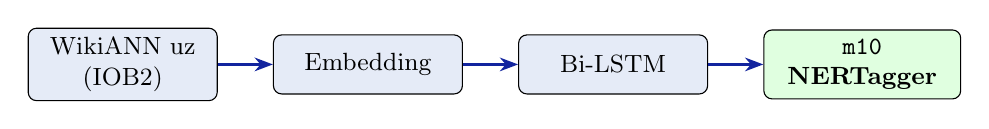
\begin{tikzpicture}[
      mod/.style={draw, fill=cnubluebg, rounded corners=3pt,
                  minimum width=2.4cm, minimum height=0.75cm,
                  font=\small, align=center},
      fin/.style={draw, fill=green!12, rounded corners=3pt,
                  minimum width=2.5cm, minimum height=0.75cm,
                  font=\small\bfseries, align=center},
      arr/.style={-{Stealth}, thick, color=cnublue}
  ]
    \node[mod] (wa) {WikiANN uz\\ (IOB2)};
    \node[mod, right=0.7cm of wa]  (em) {Embedding};
    \node[mod, right=0.7cm of em]  (bl) {Bi-LSTM};
    \node[fin, right=0.7cm of bl]  (m10) {\texttt{m10}\\ NERTagger};
    \draw[arr] (wa)--(em); \draw[arr] (em)--(bl); \draw[arr] (bl)--(m10);
  \end{tikzpicture}
  \end{center}
  \vspace{5pt}
  \begin{columns}[T]
    \begin{column}{0.50\textwidth}
      \textbf{P10 da qurasiz:}\\[3pt]
      \small
      \begin{itemize}\setlength\itemsep{2pt}
        \item \texttt{m10 NERTagger}: Embedding $+$ Bi-LSTM $+$ teg qatlami
        \item WikiANN uz da o'qitish, \texttt{seqeval} F1
        \item IOB2 teglashni tekshirish
      \end{itemize}
    \end{column}
    \begin{column}{0.46\textwidth}
      \textbf{Birinchi assert (bu slayd [I1]):}\\[4pt]
      \small\ttfamily
      assert tags ==\\
      \phantom{xx}["B-PER","B-LOC",\\
      \phantom{xx}"O","O"]\\[4pt]
      \normalfont\footnotesize\color{halfgray}
      \textit{\# Ma'ruza L10 [I1]-slayd bilan}\\
      \textit{\# solishtiring (IOB2 teglash)}
    \end{column}
  \end{columns}
\end{frame}

% ----------------------------------------------------------------
% [R] ADABIYOTLAR
% ----------------------------------------------------------------
\begin{frame}{Adabiyotlar}
  \begin{enumerate}\small\setlength\itemsep{5pt}
    \item Lample, G., va boshq.\ (2016). \textit{Neural Architectures for Named Entity
          Recognition.} NAACL-HLT 2016.
    \item Huang, Z., Xu, W., Yu, K.\ (2015). \textit{Bidirectional LSTM-CRF Models for
          Sequence Tagging.} arXiv:1508.01991.
    \item Ramshaw, L., Marcus, M.\ (1995). \textit{Text Chunking using
          Transformation-Based Learning.} (IOB sxemasi ildizi.)
    \item Pan, X., va boshq.\ (2017). \textit{Cross-lingual NER (WikiANN).} ACL 2017.
    \item \texttt{seqeval} hujjatlari --- entity-darajali NER baholash.
  \end{enumerate}
\end{frame}

% ================================================================
% [S] ILOVALAR (appendix --- slayd soniga kirmaydi)
% ================================================================
\appendix

\begin{frame}{Ilova S1: nega CRF qatlami qo'shiladi?}
  \small
  Per-token softmax teglarni \textbf{mustaqil} bashorat qiladi --- imkonsiz o'tishlarni
  (\texttt{O} $\to$ \texttt{I-LOC}) to'sa olmaydi. \textbf{CRF} (Conditional Random Field)
  butun ketma-ketlik ehtimolini modellaydi:
  $$ P(\mathbf{y}\mid\mathbf{x}) \propto \exp\Big(\sum_t \big[s(y_t,\mathbf{x}) + T(y_{t-1},y_t)\big]\Big) $$
  \bunda{$s$ --- emission balli (Bi-LSTM dan); $T(y_{t-1},y_t)$ --- teglar orasidagi
  o'tish balli (o'rganiladi); shu sababli imkonsiz o'tishlar past ball oladi.}
\end{frame}

\begin{frame}{Ilova S2: BIOES sxemasi haqida batafsil}
  \small
  IOB2 ga qo'shimcha ikki teg:
  \begin{itemize}\setlength\itemsep{2pt}
    \item \texttt{E-XXX} --- entity \textbf{oxiri} (End).
    \item \texttt{S-XXX} --- \textbf{yakka} tokenli entity (Single).
  \end{itemize}
  \bunda{"Toshkent shahri" $\to$ \texttt{B-LOC E-LOC}; "Malika" $\to$ \texttt{S-PER}.}
  \vspace{4pt}

  BIOES aniqroq chegara signali beradi (ba'zan F1 ni biroz oshiradi), ammo teglar soni
  ko'payadi $\Rightarrow$ ko'proq ma'lumot talab qiladi. Kam-resursli o'zbek uchun IOB2
  ko'pincha amaliyroq.
\end{frame}

\end{document}
